\indent Acorde a lo solicitado, mostraremos los mejores y peores casos para nuestro algoritmo, y adem\'as, daremos el tiempo estimado 
seg\'un la complejidad del algoritmo calculada anteriormente.\\

Luego de chequear varios instancias, pudimos llegar a la conclusi\'on que uno de los tipos de casos que resulta m\'as beneficioso para nuestro algoritmo
es en el cual se recibe $P$ con un valor exactamente igual a $3^i$ con 0 $\leq$ i $\leq$ n \\

Para llegar a dicha conclusi\'on trabajamos con 30 instancias ya que $3^{30}$ es el ultimo valor dentro del valor que puede tomar $P$.\\

Para una mayor observacion desarrollamos el siguiente grafico con las instancias:\\

\vspace*{0.3cm} \vspace*{0.3cm}
  \begin{center}
 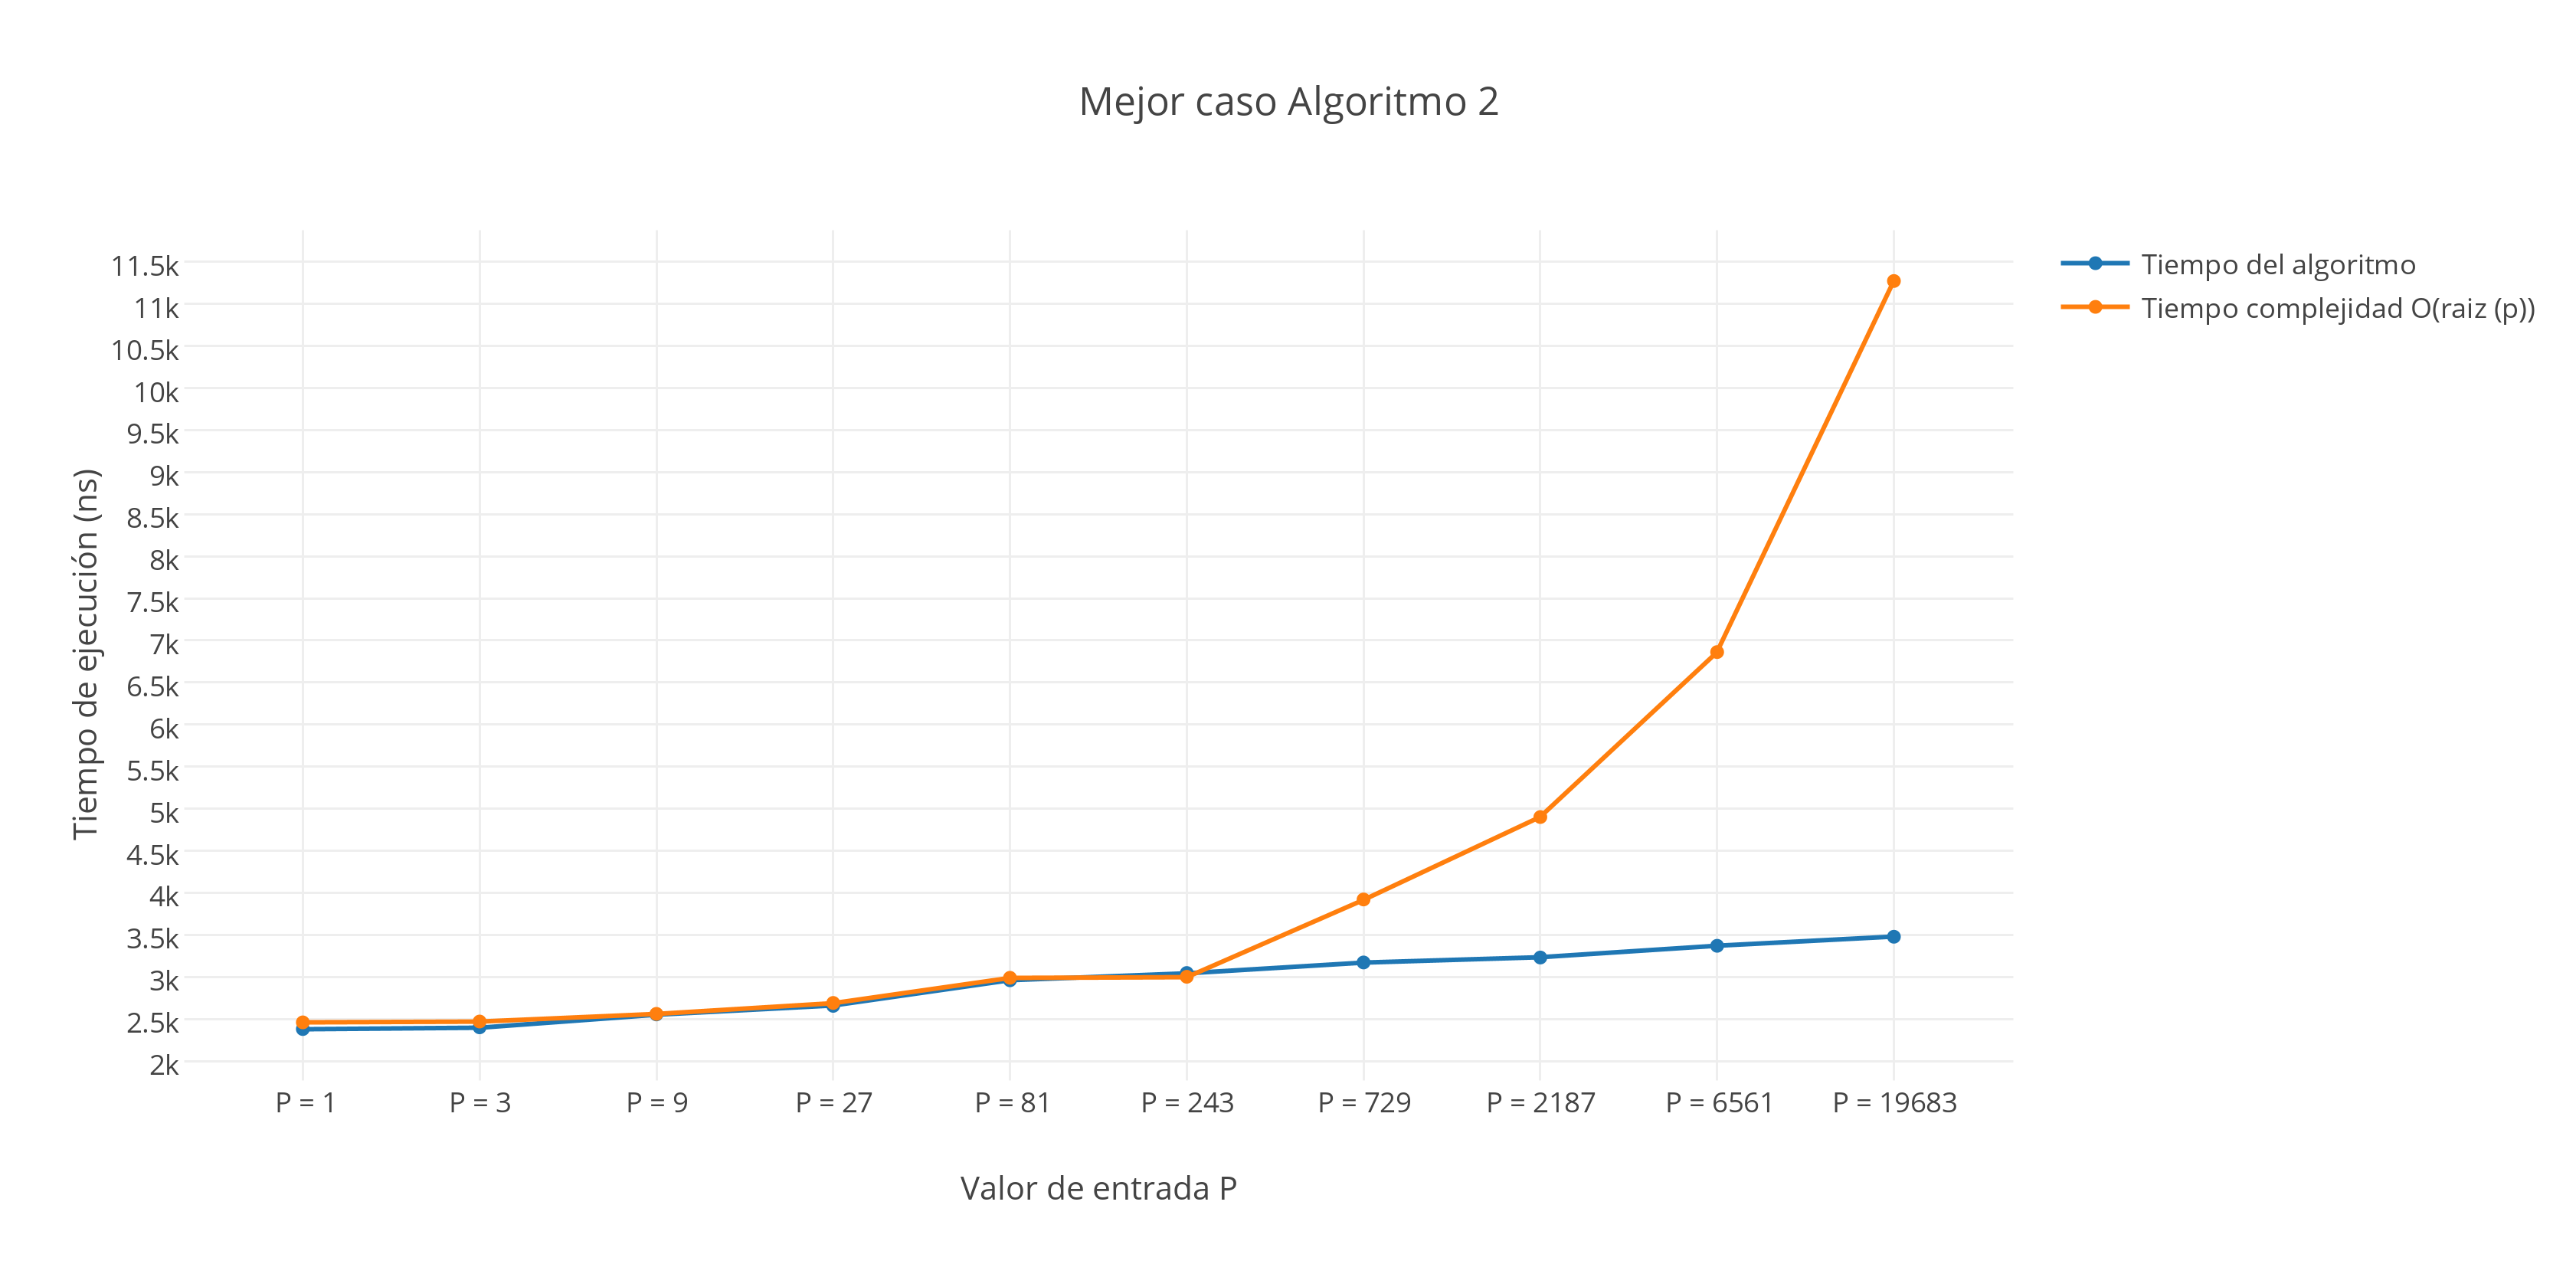
\includegraphics[scale=0.6]{./EJ2/mejorcaso.png}
  \end{center}
  \vspace*{0.3cm}
  
Y dividiendo por la complejidad de nuestro algoritmo llegamos a:\\

\vspace*{0.3cm} \vspace*{0.3cm}
  \begin{center}
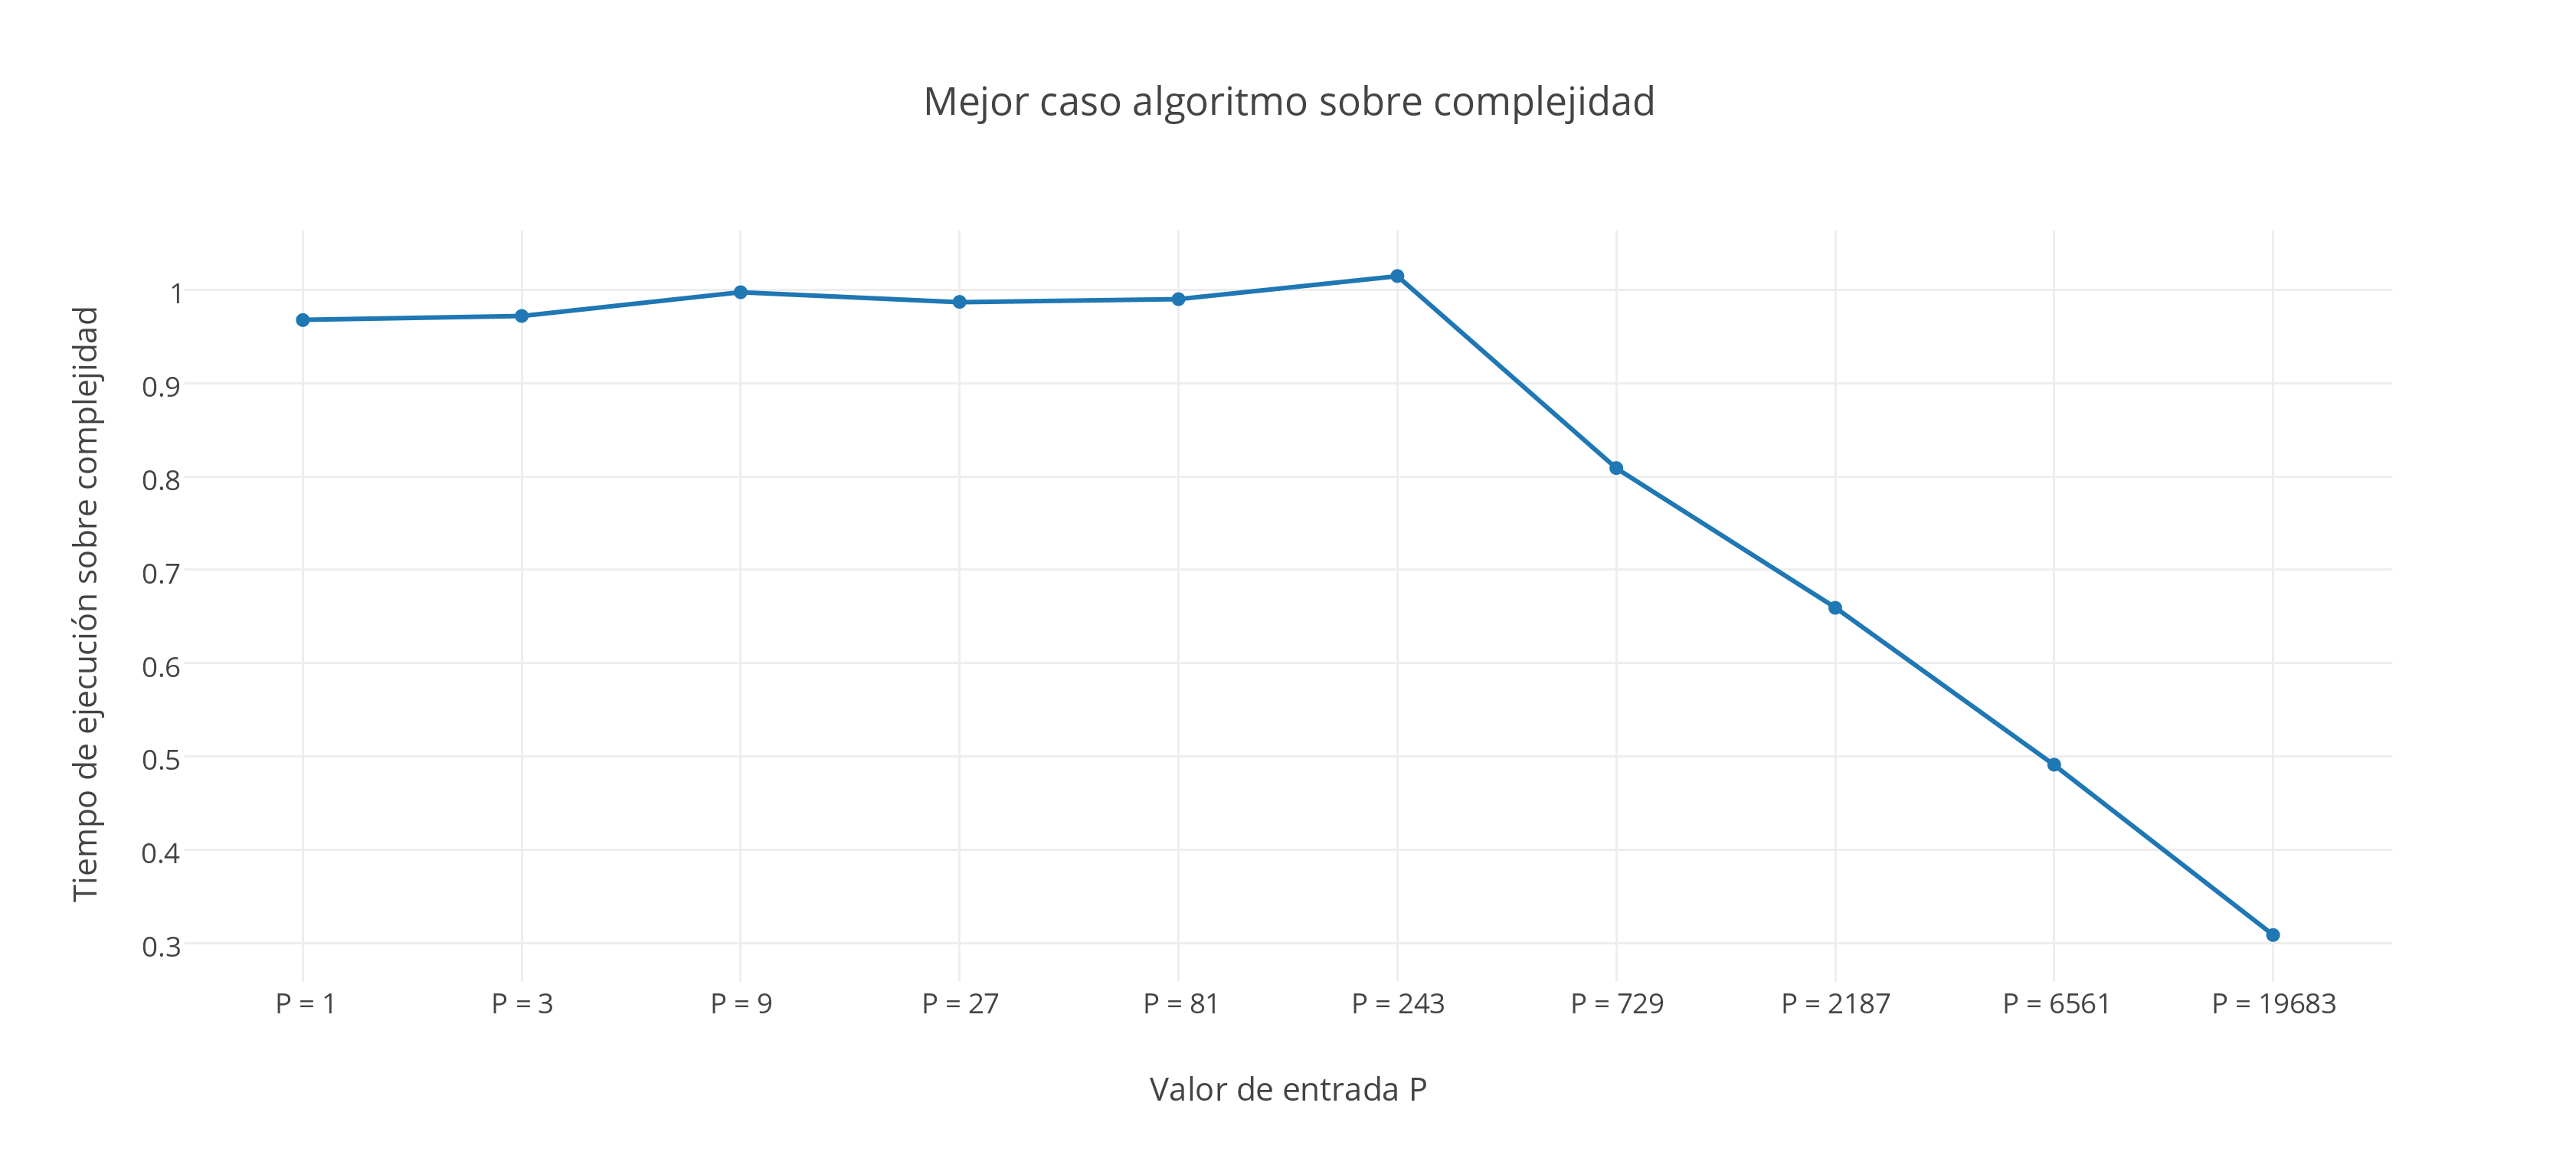
\includegraphics[scale=0.6]{./EJ2/mejorcaso2.png}
  \end{center}
  \vspace*{0.3cm}

Como se puede ver, en el primer gr\'afico cuando el valor de entrada P crece el tiempo de la funcion de la complejidad tiende a crecer muy rapido por lo cual mostraremos estas instancias en los graficos y mas adelante mostraremos una tabla con los valores restantes.\\

Para realizar esta experimentaci\'on nos parecio prudente, realizar un promedio con el mismo input de aproximadamente 20 corridas
tanto para la complejidad como para nuestro algoritmo y una vez calculado dicho promedio de ambas cosas realizamos la divisi\'on para
obtener resultados m\'as relevantes.\\ 

Se puede observar, como luego de realizar la divisi\'on por la complejidad cuando el n aumenta el valor tiende a 0.\\

A continuaci\'on mostraremos una tabla  con los 20 datos de medici\'on mas relevantes  y mostraremos un promedio de la totalidad de las instancias probadas.\\

\begin{table}[H]

    \begin{tabular}{ | l | l |l | l |}
    \hline
	Tamaño($n$) & Tiempo($t$) & \textbf{$\sqrt{P})$} & \textbf{$t/\sqrt{P})$}  \\ \hline
3$^{10}$ & 3730,82 & 18626 	& 0,2003017288 \\ \hline
3$^{11}	$ & 4428,36 & 31370 &	0,1411654447 \\ \hline
3$^{12}$ & 4685,66 & 86265  &	 0,0543170463 \\ \hline
3$^{13}	$ & 4999,42 & 124006 &	0,0403159525 \\ \hline
3$^{14}$	 & 5460,14	& 188705 & 0,0289347924 \\ \hline
3$^{15}$ & 	5756,1 & 	356824 & 0,0161314822 \\ \hline
3$^{16}$	 & 5891,5 & 265657  & 0,022177093 \\ \hline
3$^{17}	$ & 6026,9 &	400446 & 0,0150504687 \\ \hline
3$^{18}$	 & 6162,3 &	1617468 & 0,0038098435 \\ \hline
3$^{19}	$ & 6297,7 & 2542364 &	0,002477104 \\ \hline
3$^{20}$	 & 6433,1 & 2608534 &	 0,0024661745 \\ \hline
3$^{21}$ & 	6568,5 & 3956914 &	0,0016600058 \\ \hline
3$^{22}$	 & 6703,9 & 7124699 & 	0,000940938 \\ \hline
3$^{23}	$ & 6839,3 & 11467843	 & 0,0005963894 \\ \hline
3$^{24}$ & 	6974,7 & 19803192 & 	0,0003522008 \\ \hline
3$^{25}	$ & 7110,1 & 35212754 & 	0,0002019183 \\ \hline
3$^{26}$	 & 7245,5 & 59285080 & 0,0001222146 \\ \hline
3$^{27}$ &	7380,9 & 103014535 & 7,1649112428649E-005 \\ \hline
3$^{28}$	 & 7516,3 &	178188535 & 4,21817262261009E-005 \\ \hline
3$^{29}$ &	7651,7 & 308181445	& 2,48285551390026E-005 \\ \hline
3$^{30}$ &	7787,1 & 438174355 &	1,77716927317666E-005 \\ \hline

    \textbf{Promedio} & & & 0,026  \\ \hline

    \end{tabular}
\end{table}

    \textbf{Promedio total conseguido: 0,026}  \\

Verificando el peor caso, llegamos a la conclusi\'on que el tipo de caso en el que resulta menos beneficioso trabajar con nuestro algoritmo ser\'a cuando el valor de entrada $P$ sea de la forma \[
\sum_{i=1}^{n}3_{i}=P 
\].
\\

Realizando experimentos con un total de 20 instancias donde \[
\sum_{i=1}^{20}3_{i}=5230176601 
\], desarrollamos una tabla comparativa con los valores mas relevantes y ademas dos graficos los cuales mostraremos a continuaci\'on: \\

\vspace*{0.3cm} \vspace*{0.3cm}
  \begin{center}
 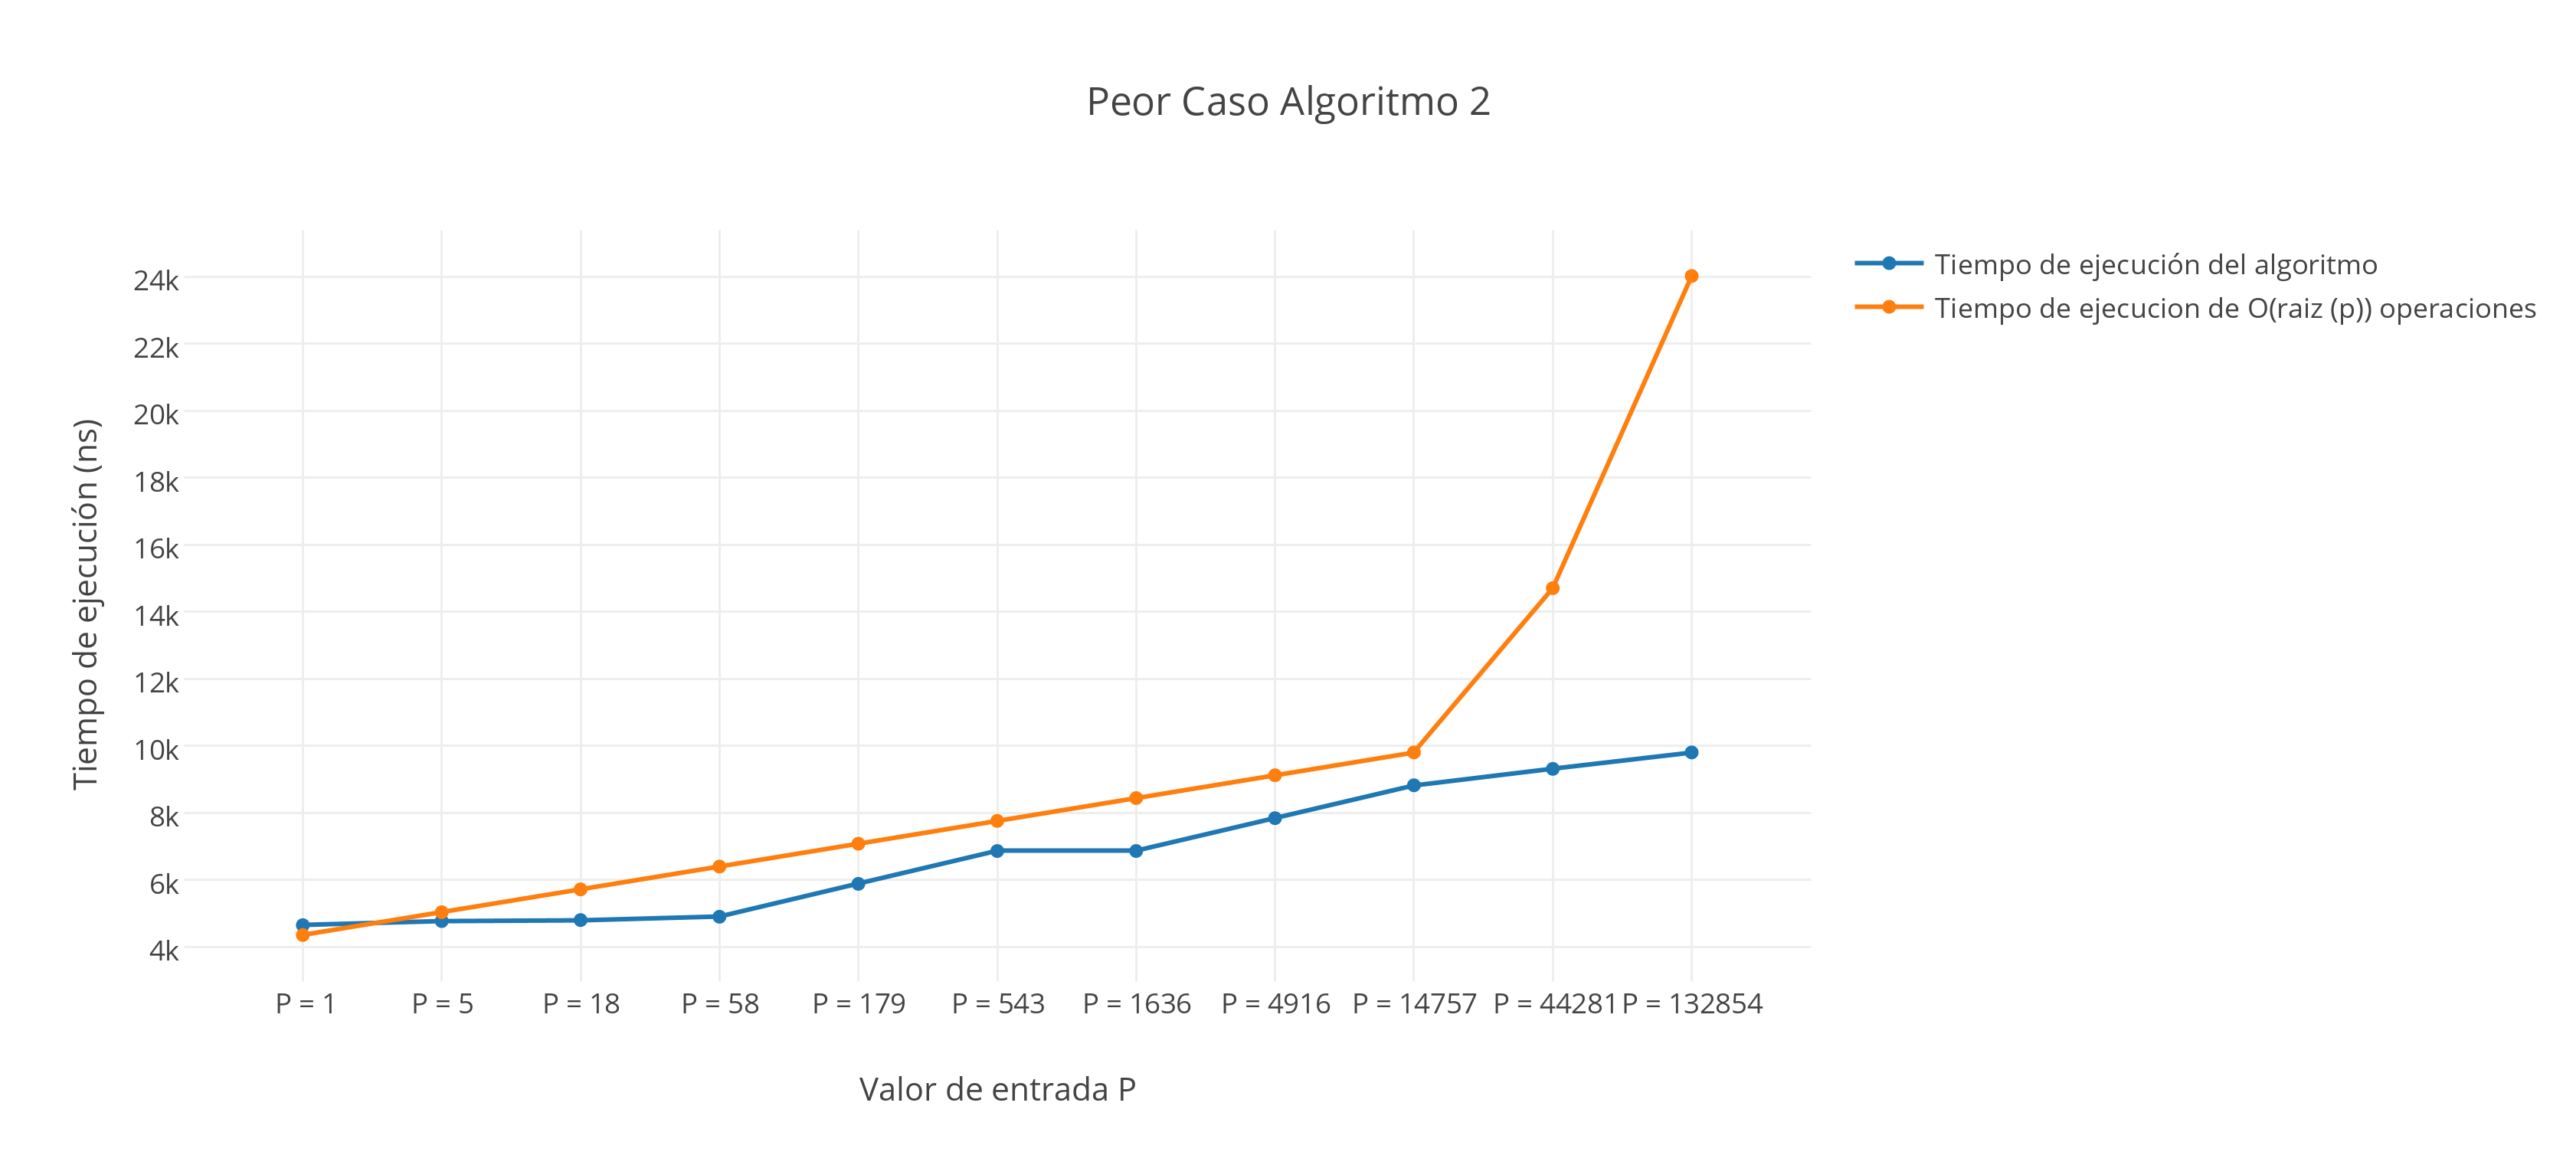
\includegraphics[scale=0.6]{./EJ2/peorcaso.png}
  \end{center}
  \vspace*{0.3cm}


Dividiendo por la complejidad propuesta llegamos a:\\

\vspace*{0.3cm} \vspace*{0.3cm}
  \begin{center}
 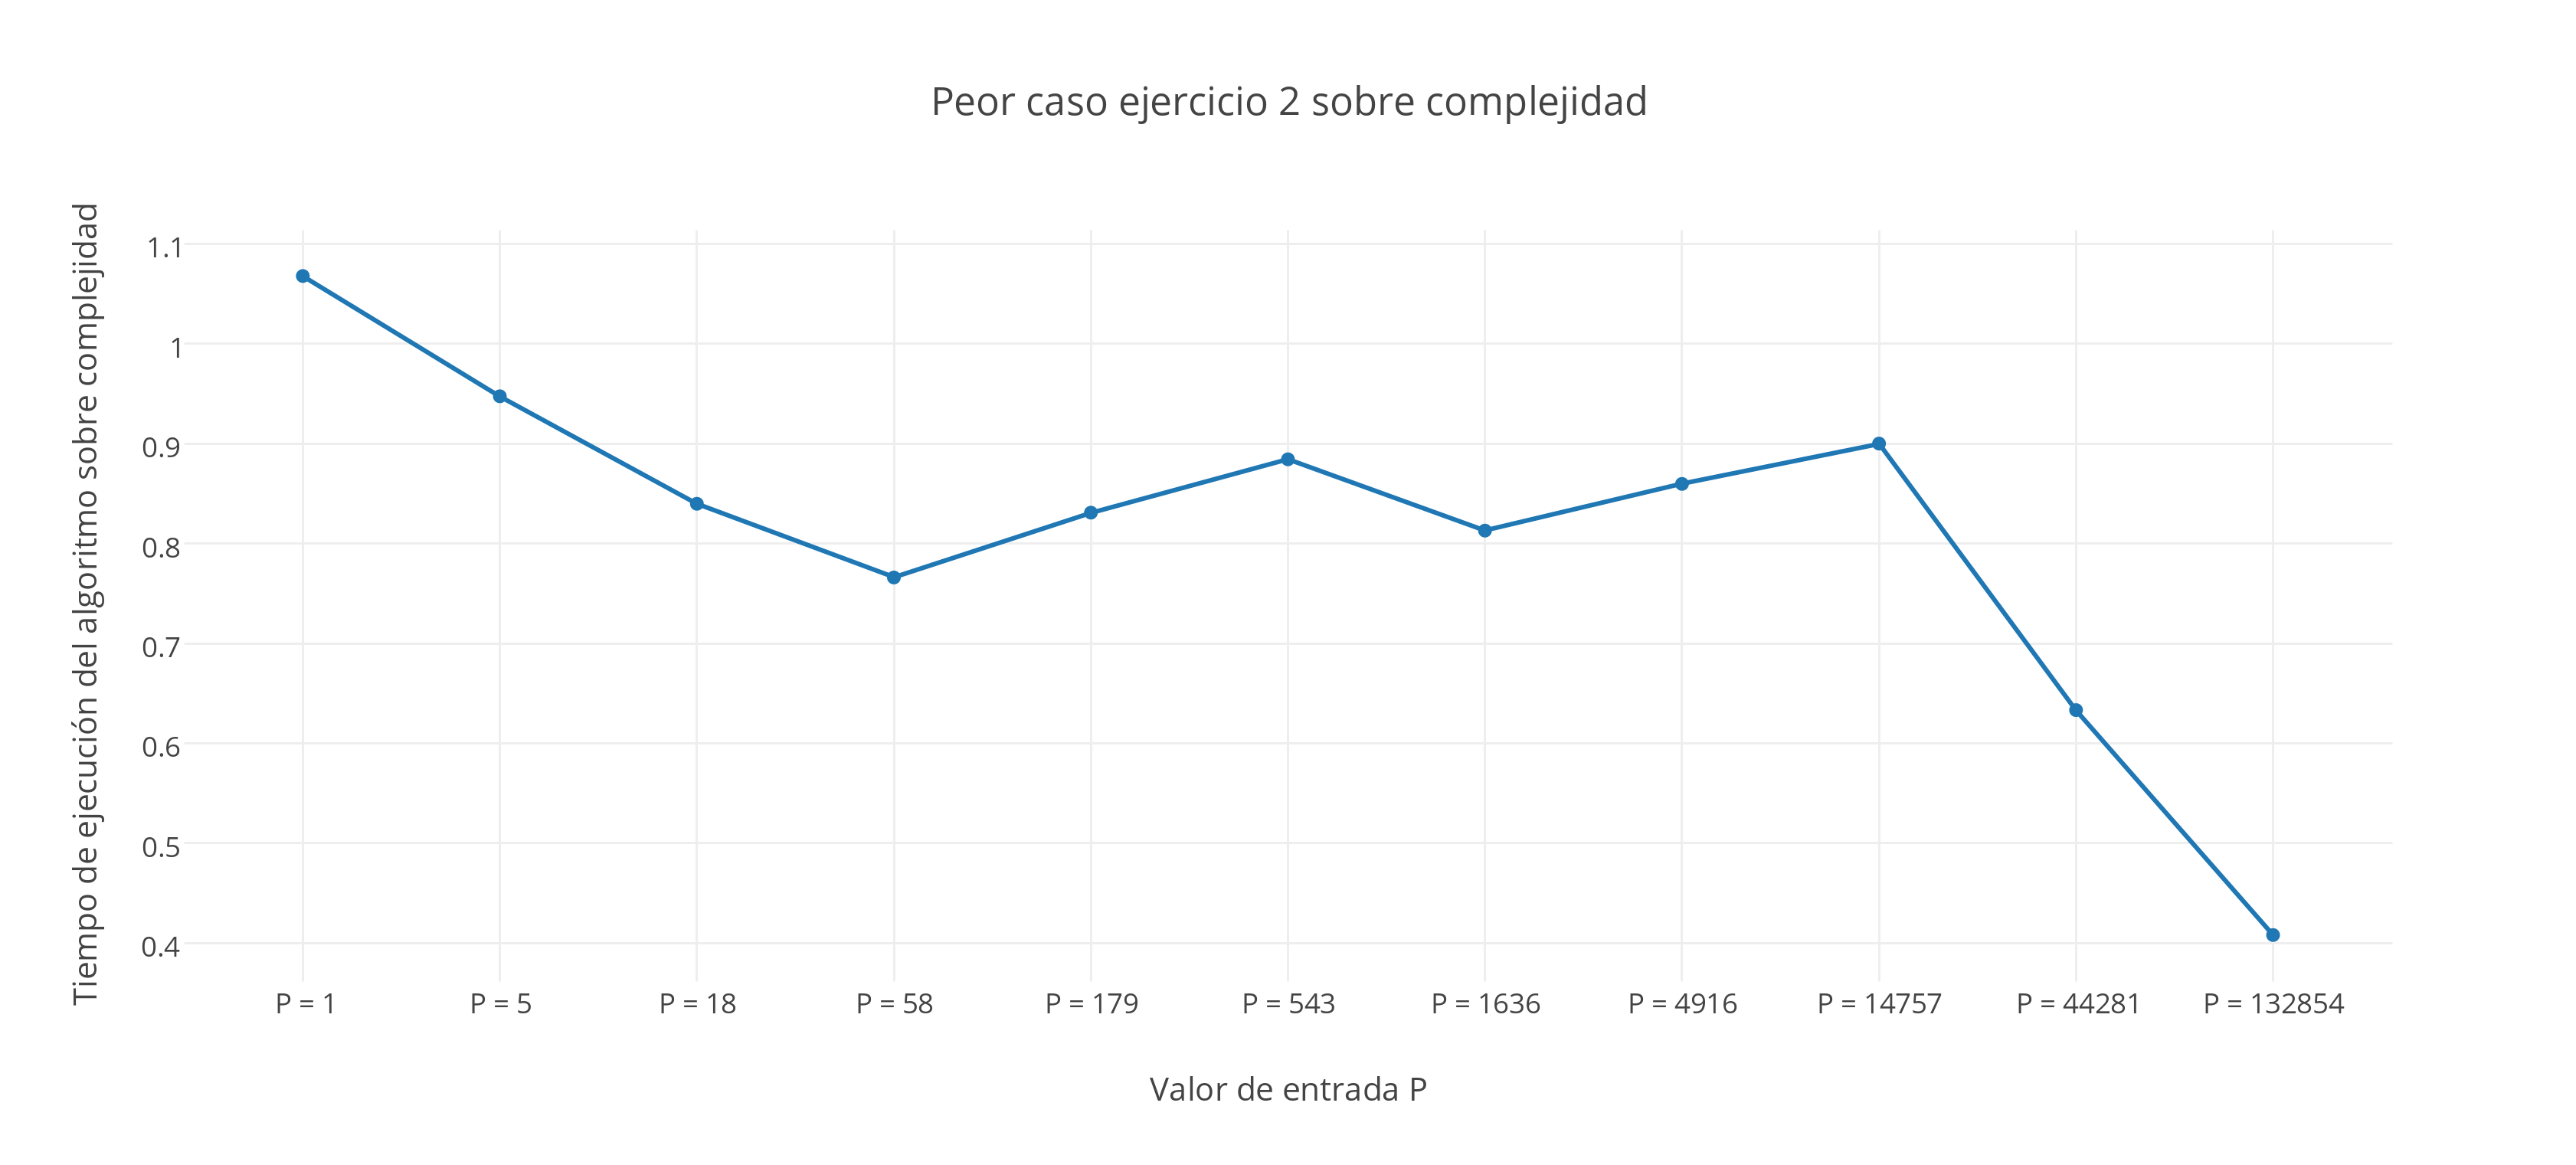
\includegraphics[scale=0.6]{./EJ2/peorcaso2.png}
  \end{center}
  \vspace*{0.3cm}

Para realizar esta experimentaci\'on nos parecio acorde, realizar un promedio con el mismo input de aproximadamente 20 corridas
tanto para la complejidad como para nuestro algoritmo y una vez calculado dicho promedio de ambas cosas realizamos la divisi\'on para
obtener resultados m\'as relevantes.\\ 

Se puede observar que a pesar de tardar varios nanosegundos este tipo de caso, al dividir por vuestra complejidad
es propenso a tender a 0 quedando comparativamente por encima del mejor caso.\\

A continuaci\'on mostraremos una tabla de valores de lass ultimas 20 instancias y
mostraremos el promedio total conseguido .\\


\begin{table}[H]

    \begin{tabular}{ | l | l |l |l |}
    \hline
	Tamaño($n$) & Tiempo($t$) & \textbf{$\sqrt{P})$} & \textbf{$t/\sqrt{P})$}  \\ \hline
1 & 4650	 & 4355 &	1.06773823191734 \\ \hline
5 &	4771	 & 5036	& 0.947378872120731\\ \hline
18 &	4801	 & 5717	& 0.839776106349484\\ \hline
58 &	4901	 & 6398	& 0.766020631447327\\ \hline
179 &	5882	 & 7079	& 0.830908320384235\\ \hline
543	& 6862	&7760 &	0.884278350515464\\ \hline
1636	6862 &	&8441 &	0.81293685582277\\ \hline
4916	7842	 & 9122 & 	 0.859679894759921\\ \hline
14757 &	8823	 & 9803 &	0.90003060287667\\ \hline
44281 &	9312	 & 14704 &	0.633297062023939\\ \hline
132854 &	 9803	 & 24017 &	0.408169213473789\\ \hline
398574 &	 18625 & 	39702 &	0.469119943579669\\ \hline
1195735 &	18625 &	67150 &	0.277364110201042\\ \hline
3587219	& 19115	& 57837&	 0.330497778238844\\ \hline
10761672 	& 26468 &	132339 & 	0.200001511270298\\ \hline
32285032	 &26468& 	 203410	& 0.130121429624896\\ \hline
96855113 & 	31860 &	307319 & 	0.103670778572103\\ \hline
290565357 &	32839 &	548960 &	 0.0598203876420869\\ \hline
581130733 & 	39211 &	910195 &	 0.0430797796076665\\ \hline
1743392200 &	41535 &	1567476 &	0.0264980133667118\\ \hline
5230176601 &	53915 &	2659024	&0.0202762366943661\\ \hline

    \textbf{Promedio} & & & 0,530 \\ \hline
    \end{tabular}
\end{table}

\textbf{Promedio total conseguido: 0,530}\\

Se puede observar como el peor caso presenta un promedio mayor que el mejor caso, concluyendo lo que enunciamos inicialmente.\\

Luego de dichos experimentos y casos probados, se puede concluir que a pesar de utilizar todas las pesas como en el peor caso nos mantenemos dentro de la complejidad propuesta como hab\'iamos mostrado en nuestro desarrollo de la complejidad.\\
